\documentclass[10pt]{beamer}
%desgin Mahdi Molavi- http://mahdimolavi.ir/
\usetheme{metropolis}
\useoutertheme{metropolis}
\useinnertheme{metropolis}
\usefonttheme{metropolis}
\usepackage{appendixnumberbeamer}
\usepackage{booktabs}
\usepackage[scale=2]{ccicons}
\usepackage{pgfplots}
\usepgfplotslibrary{dateplot}
\usepackage{xspace}
\newcommand{\themename}{\textbf{\textsc{metropolis}}\xspace}
 \usepackage{ragged2e}
\apptocmd{\frame}{}{\justifying}{} % Allow optional arguments after frame.

\usepackage{amsthm,amssymb,amsmath}
\useinnertheme{default}
\usefonttheme{professionalfonts}


\usefonttheme{serif} % default family is serif
\usepackage{hyperref}
\usepackage{xepersian}

\defpersianfont\chalkd[Scale=.8]{XM Yekan}
\DeclareMathSizes{16}{14}{12}{10}  

\settextfont[Scale=1.3]{XB Niloofar}%{HM XNiloofar}
\setlatintextfont[Scale=1.0]{Times New Roman}
%\defpersianfont\titr[Scale=1.5]{Yas}%{HM XTitr}
%\def\titr{}
%\def\parsitext#1{\rl{#1}}
\setdigitfont[Scale=1.2]{Yas}
%\setmainfont{XM Yekan}


\title{روش‌های یادگیری تانسوری}
\date{\today}
\author{مهدی مولوی، }
\institute{استاد راهنما: دکتر منصور رزقی}
% \titlegraphic{\hfill\includegraphics[height=1.5cm]{logo.pdf}}

\definecolor{blueucl}{RGB}{0,178,173} %which is the color of my university
\setbeamercolor{progress bar}{fg=blueucl,bg=red!20}
\setbeamercolor{title separator}{fg=blueucl,bg=red!20}
\setbeamercolor{progress bar in head/foot}{fg=blueucl,bg=red!20}
\setbeamercolor{progress bar in section page}{fg=blueucl,bg=red!20}

%\pgfkeys{/metropolis/.cd,
%	usetitleprogressbar/.code=\pgfkeysalso{outer/progressbar=frametitle},
%	noslidenumbers/.code=\pgfkeysalso{outer/numbering=none},
%	usetotalslideindicator/.code=\pgfkeysalso{outer/numbering=fraction},
%	nosectionslide/.code=\pgfkeysalso{inner/sectionpage=none},
%	 darkcolors/.code=\pgfkeysalso{color/background=dark},
%	blockbg/.code=\pgfkeysalso{color/block=fill, inner/block=fill},
%}


\setbeamercolor*{structure}{bg=blueucl!20,fg=blueucl}
\setbeamercolor*{palette primary}{use=structure,fg=white,bg=structure.fg}
%\setbeamercolor*{palette secondary}{use=structure,fg=white,bg=structure.fg!75}
%\setbeamercolor*{palette tertiary}{use=structure,fg=white,bg=black}
%\setbeamercolor*{palette quaternary}{fg=white,bg=black}

%\setbeamercolor{section in toc}{fg=black,bg=white}
%\setbeamercolor{alerted text}{use=structure,fg=structure.fg!50!black!80!black}
%
%\setbeamercolor{titlelike}{parent=palette primary,fg=structure.fg!50!black}
%\setbeamercolor{frametitle}{bg=myblue!85,fg=white}
%
%\setbeamercolor*{titlelike}{parent=palette primary}
\setbeamertemplate{frametitle}[default][center]

\setbeamerfont{title}{size=\LARGE,family=\chalkd,
 series=\bfseries}
 \setbeamerfont{author}{size=\LARGE,series=\normalfont,family=\chalkd}
\setbeamerfont{date}{size=\footnotesize,family=\chalkd}
% \setbeamerfont{section title}{size=\LARGE,family=\chalkd,
%series=\bfseries}
% \setbeamerfont{block title}{size=\footnotesize,family=\chalkd,
% series=\bfseries}
\setbeamerfont{standout}{size=\Huge,family=\chalkd, series=\bfseries}
% \setbeamerfont{block title alerted}{size=\normalsize,,family=\chalkd
% series=\bfseries}
% \setbeamerfont*{subtitle}{size=\footnotesize,family=\chalkd}
% \setbeamerfont{caption}{size=\small,family=\chalkd}
% \setbeamerfont{caption name}{series=\bfseries,family=\chalkd}
%\setbeamerfont{description item}{series=\bfseries}
% \setbeamerfont{page number in head/foot}{size=\scriptsize}
%\setbeamerfont{bibliography entry author}{size=\normalsize,,family=\chalkd
%	series=\normalfont}
%\setbeamerfont{bibliography entry title}{size=\normalsize,,family=\chalkd
% series=\bfseries}
% \setbeamerfont{bibliography entry location}{size=\normalsize,%
% series=\normalfont}
% \setbeamerfont{bibliography entry note}{size=\small,%
%series=\normalfont}


\setbeamerfont*{section in toc}{family=\chalkd,
	series=\bfseries}
\setbeamercolor{section in toc}{fg=black!80}
 \setbeamerfont{frametitle}{size=\Large,family=\chalkd}
 
 \useoutertheme[subsection=false]{miniframes}
 \setbeamercolor{section in head/foot}{fg=black, bg=blueucl!150}
 \setbeamerfont{section in head/foot}{size=\small,family=\chalkd}
 
 \newcommand{\normP}{$l_p$نرم }
 \newcommand{\normZero}{$l_0$نرم }
 \newcommand{\normOne}{$l_1$نرم }
 \newcommand{\normTwo}{$l_2$نرم }
 \newcommand{\trans}{\mathsf{T}}
 \newcommand\norm[1]{\left\lVert#1\right\rVert}

\setbeamertemplate{footline}[frame number]
\setbeamerfont{page number in head/foot}{size=\large,family=\chalkd}
\setbeamercolor{page number in head/foot}{fg=black, bg=blueucl!150}
\begin{document}
\linespread{1.5}
\maketitle

\begin{frame}{فهرست}

{\small
	   \setbeamertemplate{section in toc}[sections numbered]
  \tableofcontents[hideallsubsections]
}
\end{frame}
\section{مقدمه}

\begin{frame}[standout]
چند تعریف...
\end{frame}
\begin{frame}{تانسور}
\begin{center}
	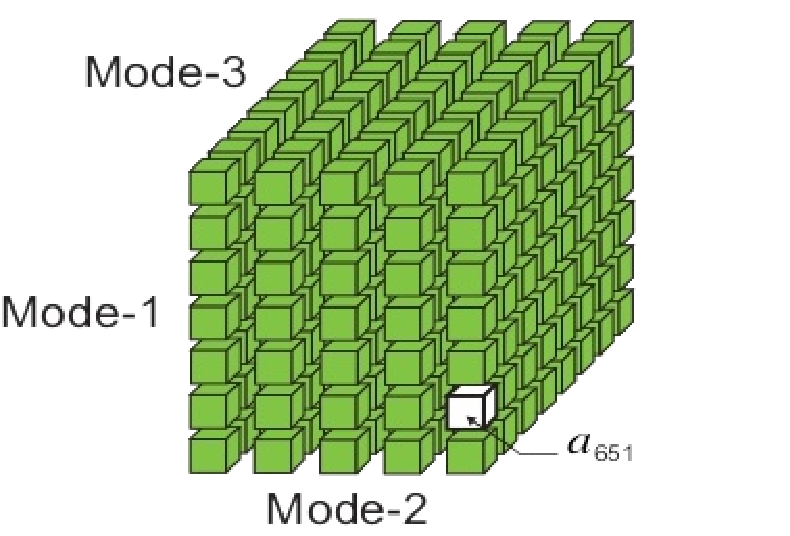
\includegraphics[width=0.5\textwidth]{img/ok/tensor3d.pdf}
\end{center}
\begin{center}
	تانسور سه بعدی
\end{center}
\end{frame}
\begin{frame}
\begin{center}
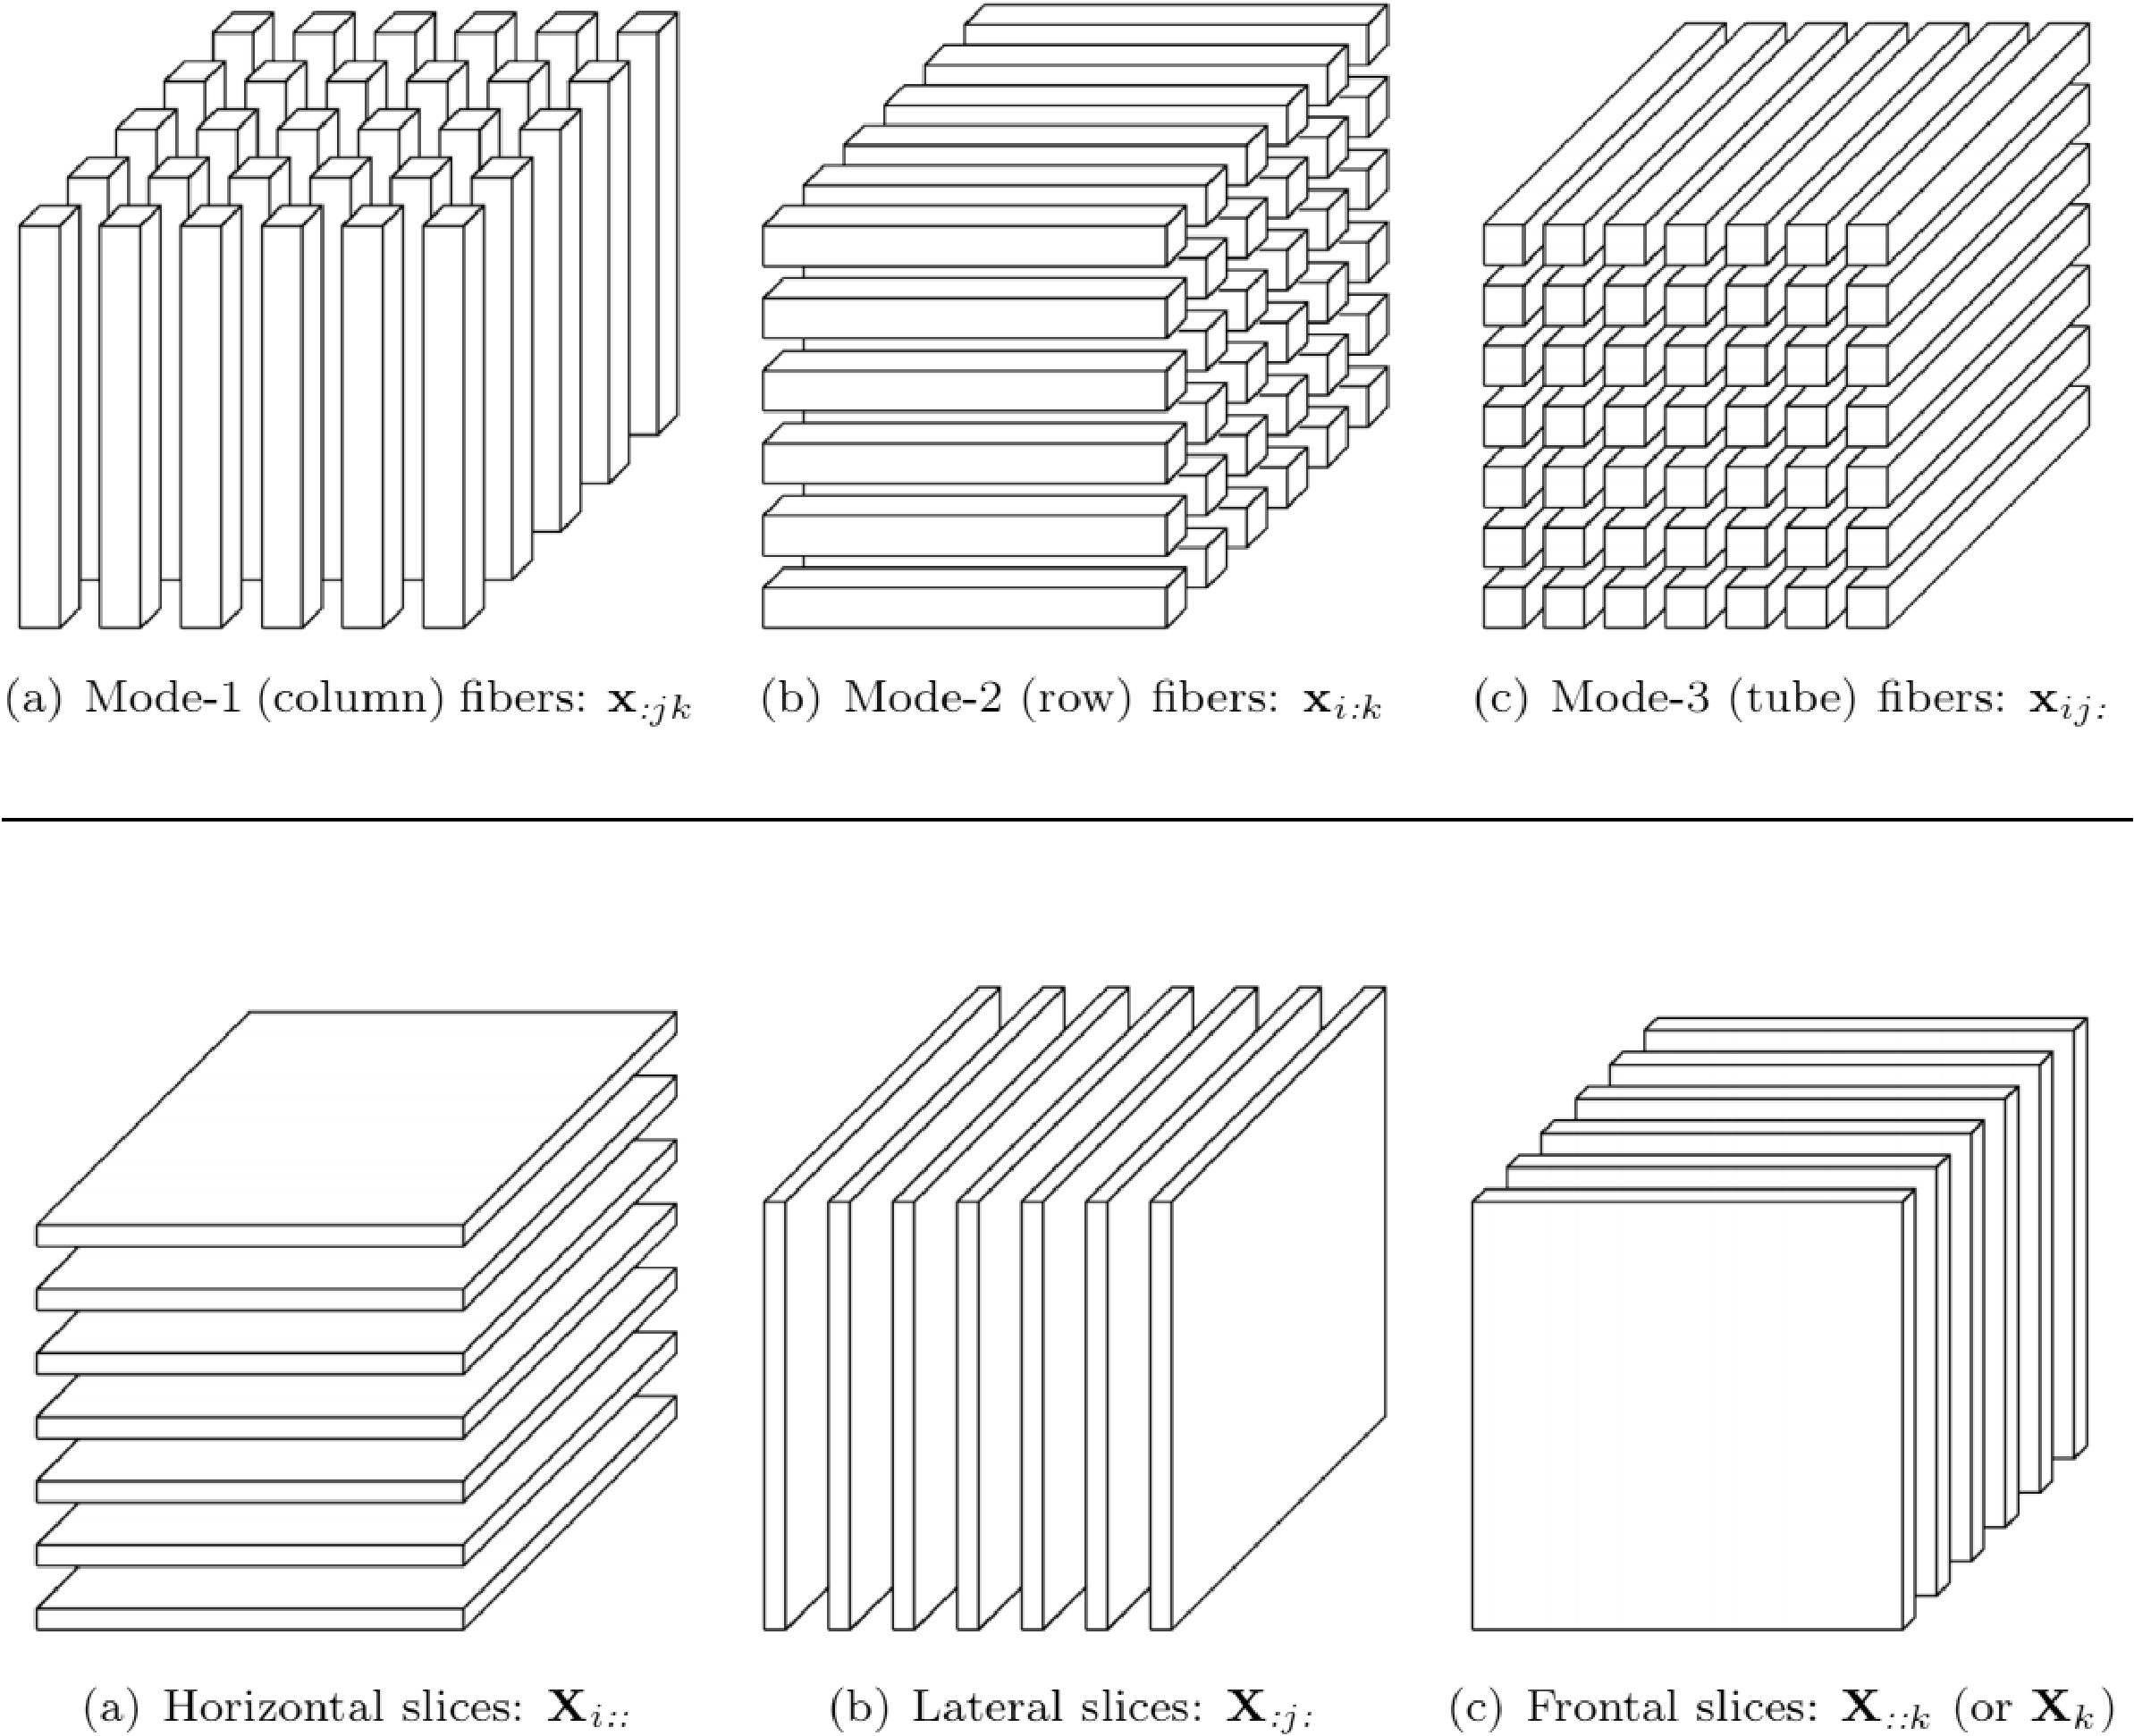
\includegraphics[width=0.9\textwidth]{img/ok/slice.pdf}
\end{center}
\end{frame}
\begin{frame}
\small{
\begin{columns}[T,onlytextwidth]
	\column{1\textwidth}	
	\metroset{block=fill}
	\begin{exampleblock}{ترانهاده ماتریس}
		ترانهاده تانسور 3-بعدی
		$\mathcal{A}\in\mathbb{R}^{n_1\times n_2\times n_3}$
		را با $\mathcal{A}^T$ نشان داده که یک تانسور با ابعاد
		$n_1\times n_2\times n_3$
		است.
		
	\end{exampleblock}\pause
	\begin{alertblock}{تانسور همانی}
		یک تانسور سه بعدی صفر را که تنها در اسلایس اولی ماتریس همانی وجود دارد را تانسور همانی گوییم.
	\end{alertblock}\pause
	\begin{block}{ضرب داخلی}
	ضرب داخلی	دو تانسور هم‌اندازه
		$\mathcal{X},\mathcal{Y}\in \mathbb{R}^{I_1\times\cdots \times I_N}$
		به‌صورت زیر تعریف می‌شود.
		\begin{center}
			\begin{tabular}{ccc}
			&$
			<\mathcal{X},\mathcal{Y}>=\displaystyle\sum_{i_1=1}^{I_1}\cdots \sum_{i_N=1}^{I_N}
			x_{i_1,i_2,\cdots,i_N}y_{i_1,i_2,\cdots,i_N}
			$&
		\end{tabular}
		\end{center}		
	\end{block}
\end{columns}
}
\end{frame}


\section{انواع تجزیه}
\begin{frame}[standout]
تجزیه CP
\end{frame}
\begin{frame}
تجزیه CP یک تانسور، مجموع اجزای رتبه یک تانسور است. به عنوان مثال؛ تانسور سه بعدی 
$\mathcal{X}\in \mathbb{R}^{I\times J\times K}$
را می‌توانیم به صورت زیر تقریب بزنیم.
\[\mathcal{X}\approx \sum_{r=1}^Ra_r \circ b_r \circ c_r,\]
که در آن $R$ یک عدد مثبت و  
$a_r\in\mathbb{R}^I$،
$b_r\in\mathbb{R}^J$
و
$c_r\in\mathbb{R}^K$
است.

\pause
\begin{center}
	\includegraphics[width=0.8\textwidth]{img/ok/cp.pdf}
\end{center}
\end{frame}

\begin{frame}
\small{
فرض کنید که هدف محاسبه بهترین تقریب برای تانسور سه بعدی 
$\mathcal{X}$
است. 

\begin{align*}
\min\limits_{\hat{\mathcal{X}}}\|\mathcal{X}-\hat{\mathcal{X}}\|
\quad \text{با}\quad
\hat{\mathcal{X}}=\sum_{r=1}^R \lambda_r a_r\circ b_r\circ c_r=[\lambda;A,B,C].
\end{align*}
که می‌توان با ثابت فرض کردن $A$ و $B$، 
برای $A$ حل کرد و همینطور به صورت تکراری برای ماتریس‌های دیگر.
}
\end{frame}
\begin{frame}[standout]
HOSVD
\end{frame}
\begin{frame}{HOSVD}
\begin{center}
	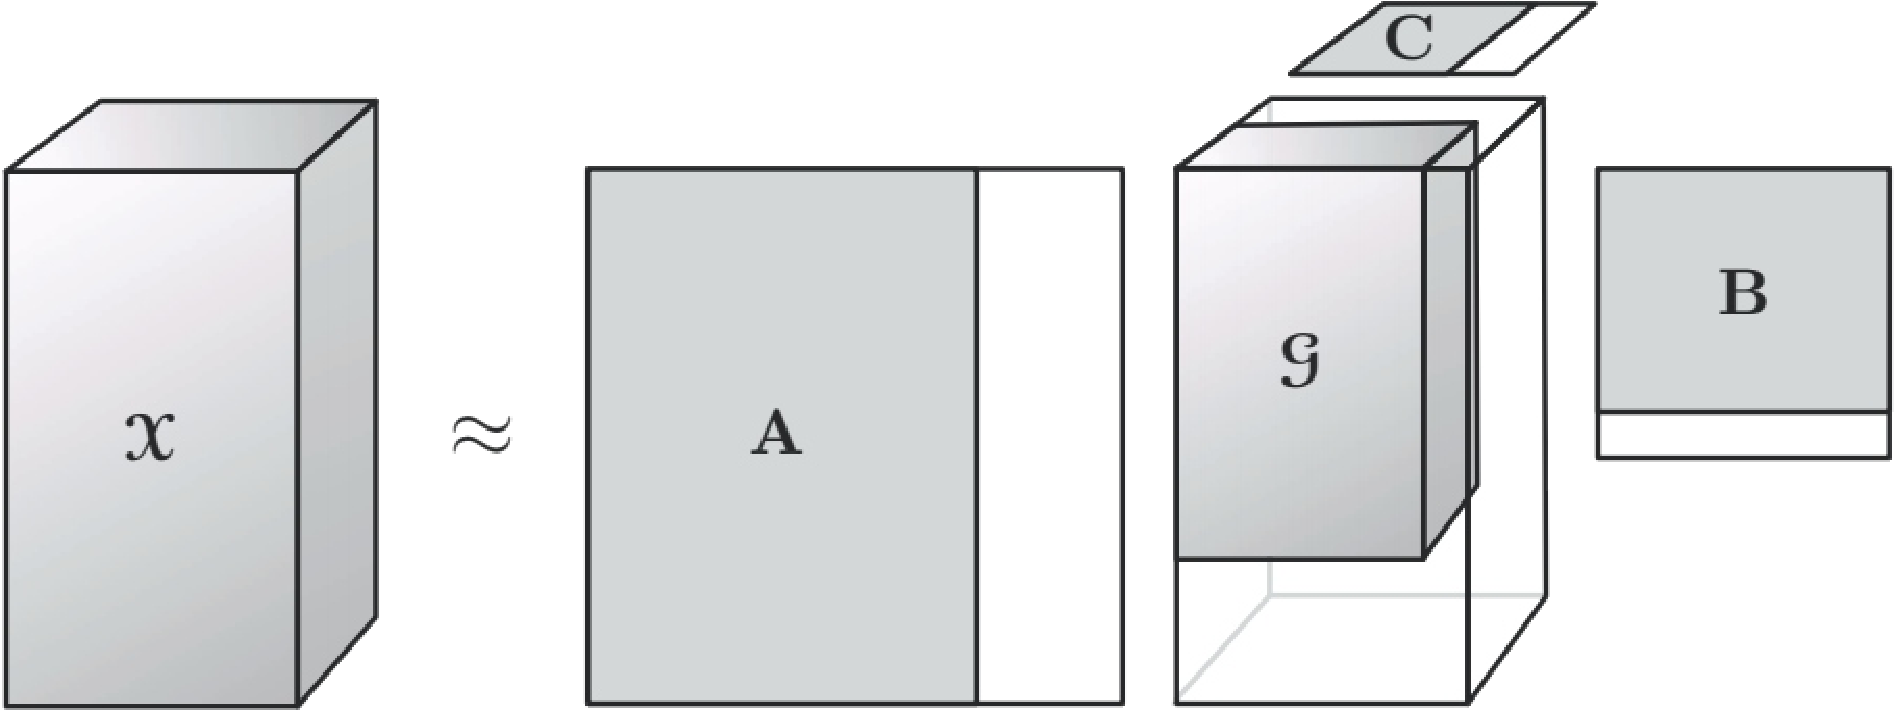
\includegraphics[width=1\textwidth]{img/ok/HOSVD.pdf}
\end{center}
\begin{center}
	تجزیه
	HOSVD
\end{center}
\end{frame}
\begin{frame}{HOSVD}
\begin{center}
	
\includegraphics[width=0.7\textwidth]{img/ok/alHOSVD.pdf}
\end{center}
\pause
\small{
هدف محاسبه مسئله بهینه سازی زیر است:
\begin{align*}
&\min\limits_{\mathcal{G},A^{(1)},\cdots,A^{(N)}} \|\mathcal{X}-[\mathcal{G};A^{(1)},\cdots,A^{(N)}]\|\\
&s.t \qquad \mathcal{G}\in\mathbb{R}^{R_1\times \cdots\times R_N}
\end{align*}
که در آن
$A^{(n)}\in\mathbb{R}^{I_n\times R_n}$
و متعامد است.
}
\end{frame}
\section{ تعمیم یادگیری‌ها به ابعاد بالاتر}
\begin{frame}[standout]
ماشین تانسور پشتیبان 
\\
\small{ تعمیم ماشین بردار پشتیبان}
\end{frame}
\begin{frame}{STM}
\small{
ماشین بردار پشتیبان از بهینه‌سازی استفاده می‌کند و  هدف آن پیدا کردن مرزهای جداسازی بهینه است. این مرز‌های بهینه با کمینه کردن خطا میان تمام مرز‌های ممکن تخمین زده شده توسط نمونه‌ها بدست می‌آید. تابع تصمیم ماشین بردار پشتیبان کلاسیک را می‌توان به صورت 
\[y(\mathrm{a}) = sign(w^\trans a + b)\]
نوشت. 
$\mathrm{a}\in \mathbb{R}^{L \times 1}$
بردار بدون برچسب ورودی، 
$y \in \{ -1,+1 \}$ برچسب حدس زده شده و
$w \in \mathbb{R}^{L \times 1}$
ماتریس تصویر است. 
}
\end{frame}
\begin{frame}{STM}
\small{
پارامتر‌های این مدل را می‌توان با حل کردن بهینه‌سازی زیر بدست آورد: 
\begin{align*}
\underset{w,b,\xi}{\min} &f(w,b,\xi) =  \frac{1}{2}\norm{w}^2 + c\sum_{i=1}^{N} \xi_i  \notag \\  
\text{\lr{s.t.}}\hspace{3mm} &y_i \left[ w^\trans \mathrm{a}_i + b \right] \geq 1 - \xi_i,\hspace{2mm}\xi_i \geq 0, \hspace{3mm} 1\leq i\leq N
\end{align*}


هدف اصلی  
\textbf{ماشین تانسور پشتیبان}
یافتن ابرصفحاتی است که داده‌های تانسوری را با توجّه به نمونه‌های آموزشی از هم جدا کند. تابع تصمیم‌گیری چندخطی برای ماشین تانسور پشتیبان،
 داده‌ی تانسوری بدون برچسب ورودی 
 \linebreak 
$\mathcal{A} \in \mathbb{R}^{I_1 \times I_2 \times \cdots I_N}$،
به صورت 
\begin{align*}
y(\mathcal{A}) = sgn \left(  \mathcal{A} \prod_{k=1}^{N} \times_k w_k + b \right)
\end{align*}
تعریف  می‌شود. که در آن 
$y \in \{ +1,-1 \}$،
$b$
است.
}
\end{frame}
\begin{frame}{STM}
\small{
	وزن‌های
$w_k$
 به صورت زیر محاسبه می‌شود: 
\begin{align}\label{STM_Primal}
\underset{w_k |_{k=1}^{N}}{\min} &f\left( w_k |_{k=1}^{N}, b, \xi\right) = \frac{1}{2} \|{ w_1 \circ w_2 \circ \cdots \circ w_N }\|^2 + c\sum_{i=1}^{N} \xi_i\\
\text{\lr{s.t.}}\hspace{3mm} & y_i \left[ \mathcal{A}_i \prod_{k=1}^{N} \times_k w_k + b \right] \geq 1 - \xi_i, 1\leq i\leq M , \hspace{3mm}\xi_i \geq 0 \notag
\end{align}

\pause
که در آن 
$w_k |_{k=1}^{N}$
 بیانگر وزن در حالت 
$k$ام
است. در این معادله، 
$\xi_i$
بردار متغیّر اسلک بوده و 
$c$
ضریب منظّم‌ساز برای کنترل خطا‌های طبقه‌بندی است. همچنین 
$M$
تعداد کلّ نمونه‌ها و 
$\mathcal{A}_i$ 
نشان‌دهنده‌ی 
$i$امین
تانسور داده‌های آموزشی است. 
}
\end{frame}
\begin{frame}{STM}
\small{
 	می‌توان از روش‌های 
	\textit{متناوب}
	برای پیدا کردن جوابی مناسب استفاده کرد. گرچه این روش‌ها تضمینی برای رسیدم به نقطه‌ی کمینه به ما نمی‌دهند اما ثابت شده که همواره به یک نقطه‌ی کمینه‌ی محلی خواهند رسید. پس از محاسبه‌ی 
	$w_j$ و
	$b$
	می‌توان ابرصفحه‌ی جداساز را با استفاده از رابطه‌ی زیر محاسبه کرد:
	
	\pause
	\begin{align*}
	\mathcal{A}\prod_{k=1}^{N} \times_k w_k + b = 0.
	\end{align*}
}
\end{frame}
\begin{frame}
\small{
	نمایی از جداسازی دودویی  به وسیله‌ی ماشین تانسور پشتیبان در فضای با ابعاد بالا 

}
	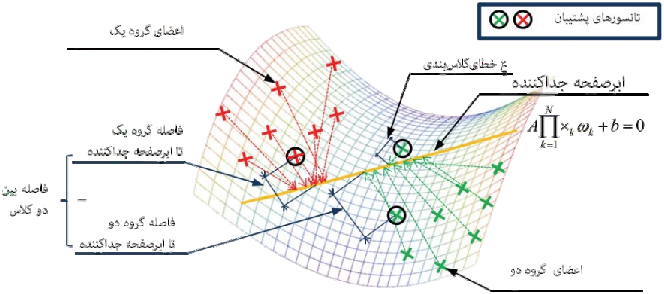
\includegraphics[width=1\textwidth]{img/ok/STM.pdf}

\end{frame}
\begin{frame}[standout]
Tensor Spectral Clustering
\end{frame}
\begin{frame}[standout]
Logistic Tensor Regression
\end{frame}

\section{سرعت بخشی}
\begin{frame}[standout]
\begin{latin}
	HOSVD for Dimensionality Reduction
	\end{latin}
\end{frame}
\begin{frame}
{مقدمه}
\small{
فرض کنید 
$M_1\in \mathbb{R}^{m_1\times n}$
و
$M_2\in \mathbb{R}^{m_2\times n}$
که 
$m_1<m_2$
است و 
$M_2=[M_1,~~0]$.

هرگاه تجزیه $SVD$ آن‌ها به صورت زیر باشد:
\begin{align*}
M_1=&U_1\Sigma_1V_1^T\\
M2=&U_1\Sigma_1V_1^T
\end{align*}
در این صورت ماتریس متعامد $U_1$ معادل با $U_2$ است.

\pause
\textbf{نتیجه:}
فرض کنید 
$M_1=[v_1,\cdots,v_n]$
و
$M_2=[v_1,v_2,\cdots,0,\cdots,0,v_n]$،
در این صورت پایه‌هی معادل دارن.
}
\end{frame}
\begin{frame}{معادل بودن تانسوری هسته در $HOSVD$}
فرض کنید 
$T\in \mathbb{R}^{I_1\times\cdots I_N}$
و
$G\in \mathbb{R}^{I_1\times\cdots\times(kI_n)\times\cdots I_N}$
باشد.
با در نظر گرفتن ماتریس
\[
M=\begin{pmatrix}
I\\0
\end{pmatrix},\qquad M\in\mathbb{R}^{I_n\times (kI_n)}
\]
تانسور  $T$ و $G$ در رابطه زیر صدق می‌کند:
\[T=G\times_nM=G\times_n\begin{pmatrix}
I_n\\0_{kn}
\end{pmatrix},\]
\end{frame}
\begin{frame}{IHOSVD}
این روش شامل سه الگوریتم است که در اولین الگوریتم، یک الگوریتم بازگشتی می‌باشد که تابع زیر را بدست می‌آورد:
\begin{align*}
f(M_n,C_n)=
\begin{cases}
svd(M_1),& n=1\\
mix(f(M_{n-1},C_{n-1}),C_n),&n>1
\end{cases}
\end{align*}
\end{frame}
\begin{frame}{IHOSVD}
\begin{center}
	
\includegraphics[width=.8\textwidth]{img/ok/AIHOSVD.pdf}
\end{center}
\end{frame}
\begin{frame}{IHOSVD}
دومین الگوریتم، $SVD$ را بروزرسانی می‌کند. از ورودی ماتریس $C_{n-1}$ را خوانده و به فضای متعامد تولید شده از $U_m$ تصویر می‌کند.
\begin{center}
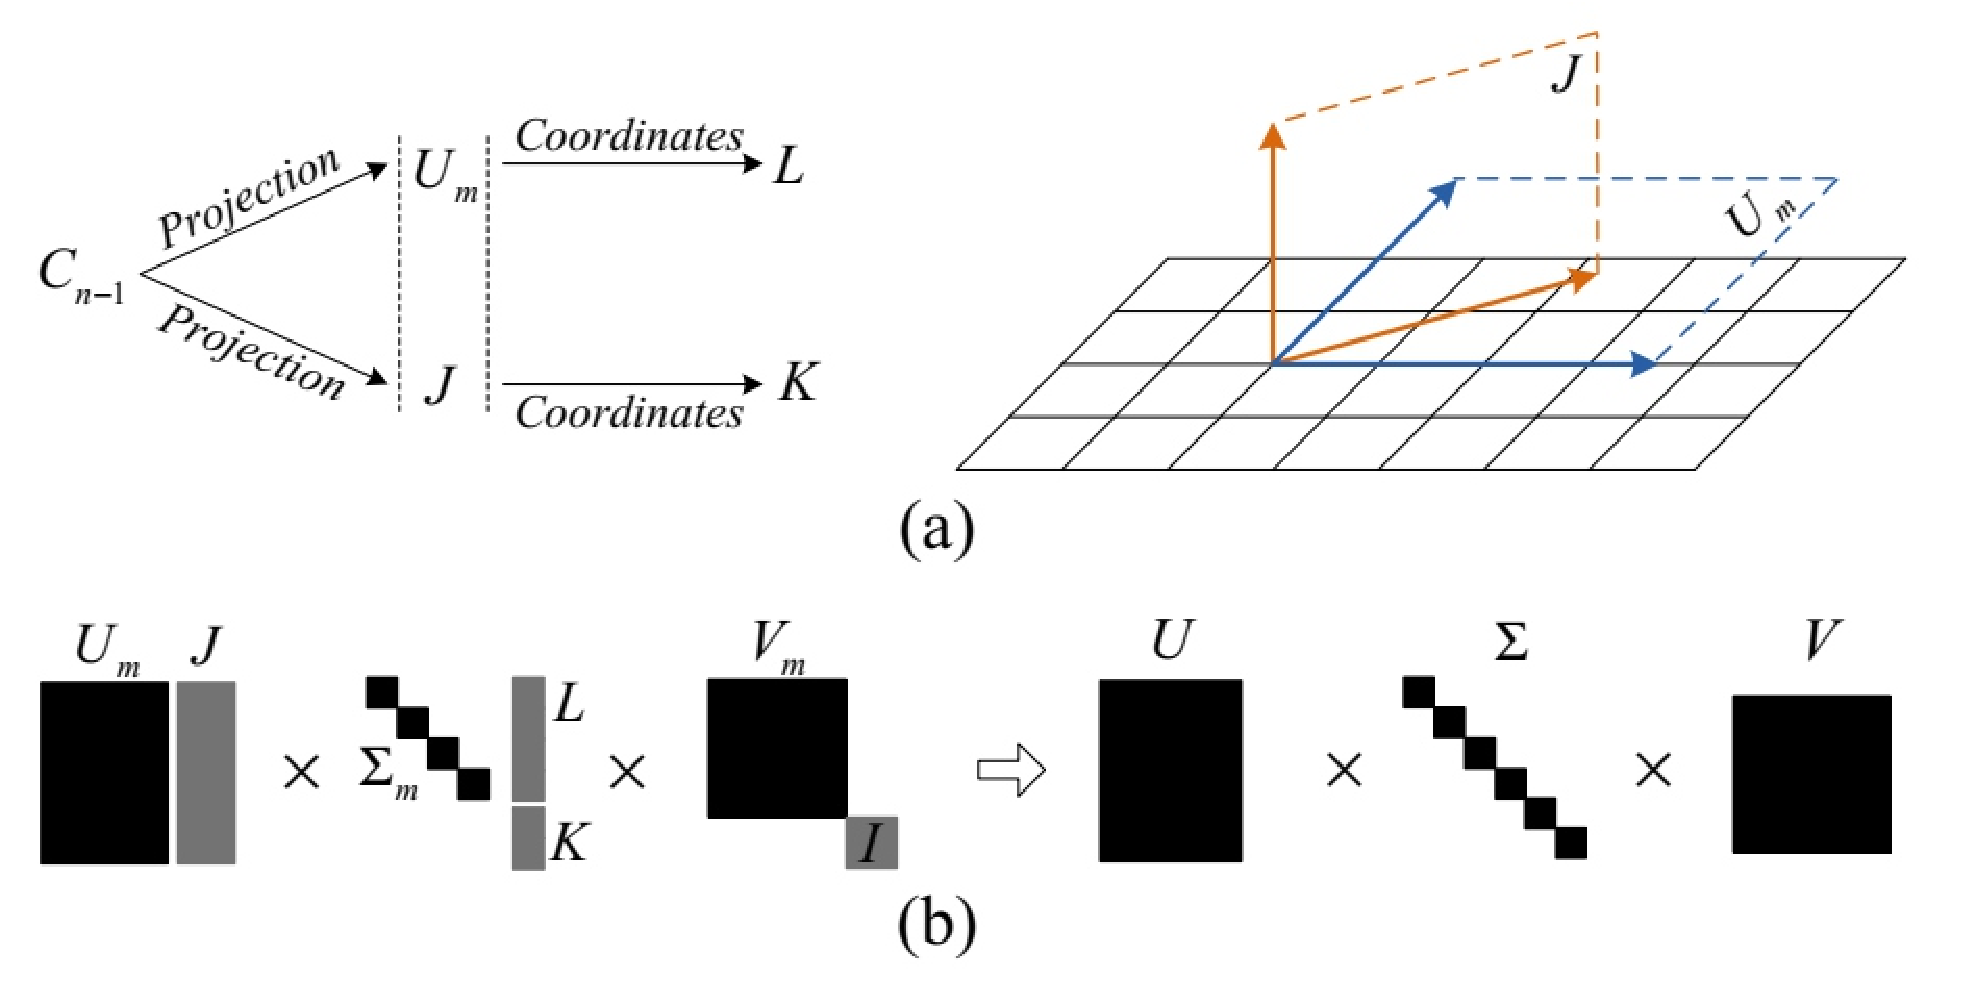
\includegraphics[width=.8\textwidth]{img/ok/fig8.pdf}
\end{center}
\end{frame}
\begin{frame}
\begin{center}

\includegraphics[width=.8\textwidth]{img/ok/AIHOSVD2.pdf}
\end{center}
\end{frame}
\begin{frame}{IHOSVD}
با استفاده از سومین الگوریتم  ما هسته تانسور را حساب خواهیم کرد.

\pause
\begin{center}
	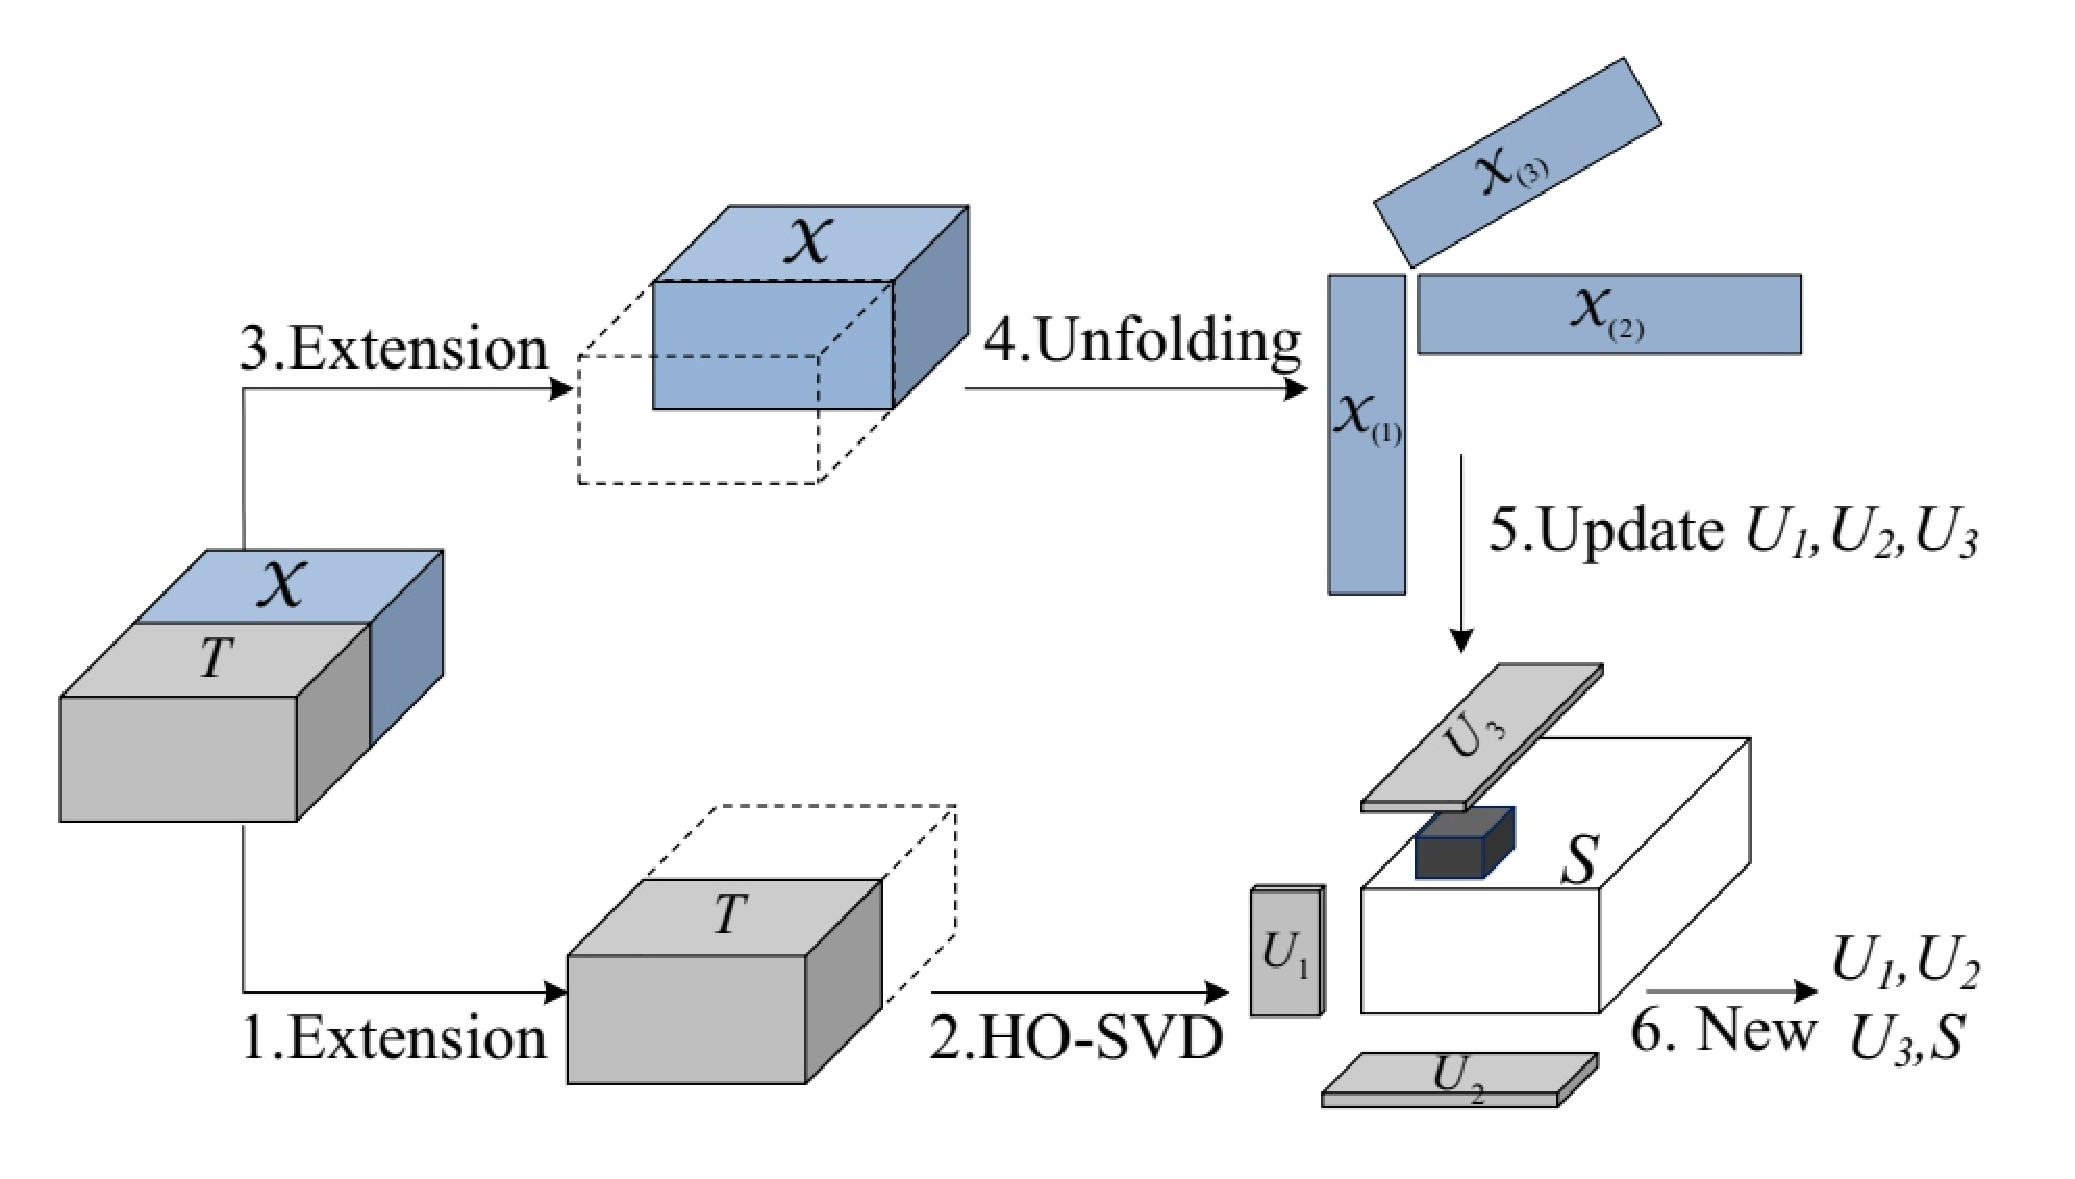
\includegraphics[width=.8\textwidth]{img/ok/AIHOSVD3.pdf}
\end{center}
\end{frame}
\begin{frame}
\begin{center}
	
\includegraphics[width=.8\textwidth]{img/ok/AIHOSVD4.pdf}
\end{center}
\end{frame}
\begin{frame}{زمان پیچیدگی}
\small{
زمان محاسبه برای روش ارائه شده به صورت مجموع سه الگوریتم است که به صورت زیر محاسبه می‌شود:
\[Time=Time_{unf}+Time_{isvd}+Time_{prod}.\]
که عمله تبدیل unfolding  یک عمل از مرتبه 
$\mathcal{O}(1)$
است. زمان $Time_{isvd}$ مجموع زمان‌های مصرفی برای unfold کردن ماتریس $T_{(i)}$ است.
\begin{align*}
Time_N&=\sum_{i=1}^N Time_i\\
Time(n)&=\begin{cases}
C_1,&n=1\\
Time(n-1)+C_2,&n>1
\end{cases}
\end{align*}
پس زمان کل برابر $\mathcal{O}(k^2n)$ است.

}
\end{frame}
\section{رویکرد دیگر برای تجزیه SVD برای ابعاد بالاتر}
\begin{frame}[standout]
T-SVD
\end{frame}
\begin{frame}
{تعاریف مقدماتی}
\metroset{block=fill}
 \begin{alertblock}{ماتریس پیچشی}
	 تانسور سه بعدی
	$\mathcal{A}\in\mathbb{R}^{l\times m\times n}$
	با $l\times m$ اسلایس پیشی مفروض است. در این صورت
	\begin{tabular}{p{0.7cm}cc}
	 	&
	$
	circ(\mathcal{A})=\begin{pmatrix}
	A^{(1)}&A^{(n)}&A^{(n-1)}&\cdots &A^{(2)}\\
	A^{(2)}&A^{(1)}&A^{(n)}&A^{(n-1)}&\cdots \\
	\vdots &\ddots&\ddots&\ddots&\vdots\\	
	A^{(n)}&A^{(n-1)}&\cdots &A^{(2)}&A^{(1)}\\
	\end{pmatrix}
	$
	&
\end{tabular}
که ماتریس پیچشی بلوکی از سایز 
$ln\times mn$
است.
\end{alertblock}
\end{frame}
\begin{frame}{T-Prudact}
\metroset{block=fill}
\begin{exampleblock}{عملگرهای $fold$ و $MatVec$}
	عملگر $MatVec$ تانسور سه بعدی به ابعاد 
	$l\times m\times n$
	را به ماتریس بلوکی با ابعاد 
	$ln \times m$
	برمی‌گرداند و عملگر $fold$ معکوس این عملگر را انجام می‌دهد.
	
	\begin{tabular}{p{0.9cm}ccc}
&$	MatVec(\mathcal{A})=\begin{pmatrix}
A^{(1)}\\A^{(2)}\\\vdots\\ A^{(n)}\\
\end{pmatrix}$&
$fold(MatVec(\mathcal{A}))=\mathcal{A},$&
	\end{tabular}
\end{exampleblock}
\end{frame}
\begin{frame}
\small{
\metroset{block=fill}
\begin{alertblock}{$t$-ضرب}
	فرض کنید 
	$\mathcal{A}\in \mathbb{R}^{l\times p\times n}$
	و
	$\mathcal{B}\in \mathbb{R}^{p\times m\times n}$.
	در این صورت $t$-ضرب با ابعاد
	$l\times m\times n$
	را به صورت 
	$\mathcal{A} \star \mathcal{B}$
	نشان داده و به صورت زیر تعریف می‌شود.
	
	\begin{tabular}{p{1.3cm}cc}
		&$\mathcal{A} \star \mathcal{B}=fold\left(circ(\mathcal{A}) MatVec(\mathcal{B})\right).$
	\end{tabular}

\pause
این ضرب در حالت کلی خاصیت جابجایی ندارد.
\end{alertblock}

\pause
\metroset{block=fill}
\begin{alertblock}{تبدیل فوریه گسسته ($DFT$)}
	ماتریس مربعی $F$ با ابعاد $N$ در $N$ را به صورت
	$F=\left(\frac{w^{jk}}{\sqrt{N}}\right)_{j,k=0,\cdots,N-1}$
	که در آن
	$\omega=e^{-2\pi i/N}$ 
	است.
	 به صورت ماتریس داریم:	
	\begin{center}
		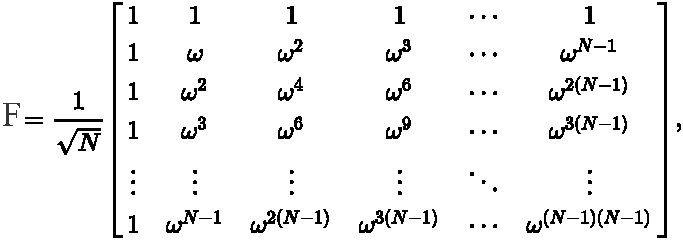
\includegraphics[width=0.5\textwidth]{img/ok/DFTW.pdf}
	\end{center}
\end{alertblock}
}
\end{frame}
\begin{frame}{T-SVD}
هرگاه $F$ ماتریس نرمال شده تبدیل فوریه باشد، برای 
$\mathcal{A}\in \mathbb{R}^{l\times m\times n}$،
$n$
ماتریس با درآیه‌های مختلط
$\hat{A}^{(i)}$
با ابعاد 
$l\times m$
وجود دارد به طوریکه:
\[(F\otimes I)circ(\mathcal{A})(F^*\otimes I)=
\begin{pmatrix}
\hat{A}^{(1)} & 0 &\cdots & 0\\
0&\hat{A}^{(2)}&\cdots & 0\\
\vdots&\ddots&\ddots&\vdots\\
0&0&\cdots&\hat{A}^{(n)}
\end{pmatrix}=\hat{\mathcal{A}},
 \]
 اما نیاز نیست که به صورت صریح
 $\hat{\mathcal{A}}$
 از 
 $circ(\mathcal{A})$
 تولید شود. با  تبدیل فوریه  از مد سوم تانسور $\mathcal{A}$
 تانسور 
  $\hat{\mathcal{A}}$،
  تولید می‌شود.
  
  \pause
  توجه: برای تانسور $\mathcal{A}$ و $\mathcal{B}$
  داریم:
  \[\mathcal{A}\star \mathcal{B}=\mathcal{C} \Longleftrightarrow \hat{\mathcal{A}}\hat{\mathcal{B}}=\hat{\mathcal{C}} \]
\end{frame}
\begin{frame}{T-QR and T-SVD}
\metroset{block=fill}
\begin{alertblock}{تجزیه $T-QR$}
	با استفاده از تعریف فوق می‌توان تانسور $\mathcal{A}$ را بصورت
	$\mathcal{A}=\mathcal{Q}\star \mathcal{R}$
	نوشت که در آن
	$\mathcal{Q}$
	معکوس تبدیل فوریه 
	$\hat{\mathcal{Q}}$
	مد 3 است.
\end{alertblock}

\pause
\metroset{block=fill}
\begin{exampleblock}{تجزیه $T-SVD$}
با استفاده از تعریف  می‌توان تانسور $\mathcal{A}$ را بصورت
$\mathcal{A}=\mathcal{U}\star\mathcal{S}\star \mathcal{V}^\trans$
نوشت.
\end{exampleblock}
\end{frame}
\begin{frame}{T-SVD}
تجزیه $t-SVD$ که در آن $\mathcal{S}$ 
تانسور قطری است به فرم زیر نشان داده می‌شود.

\pause
	\begin{center}
	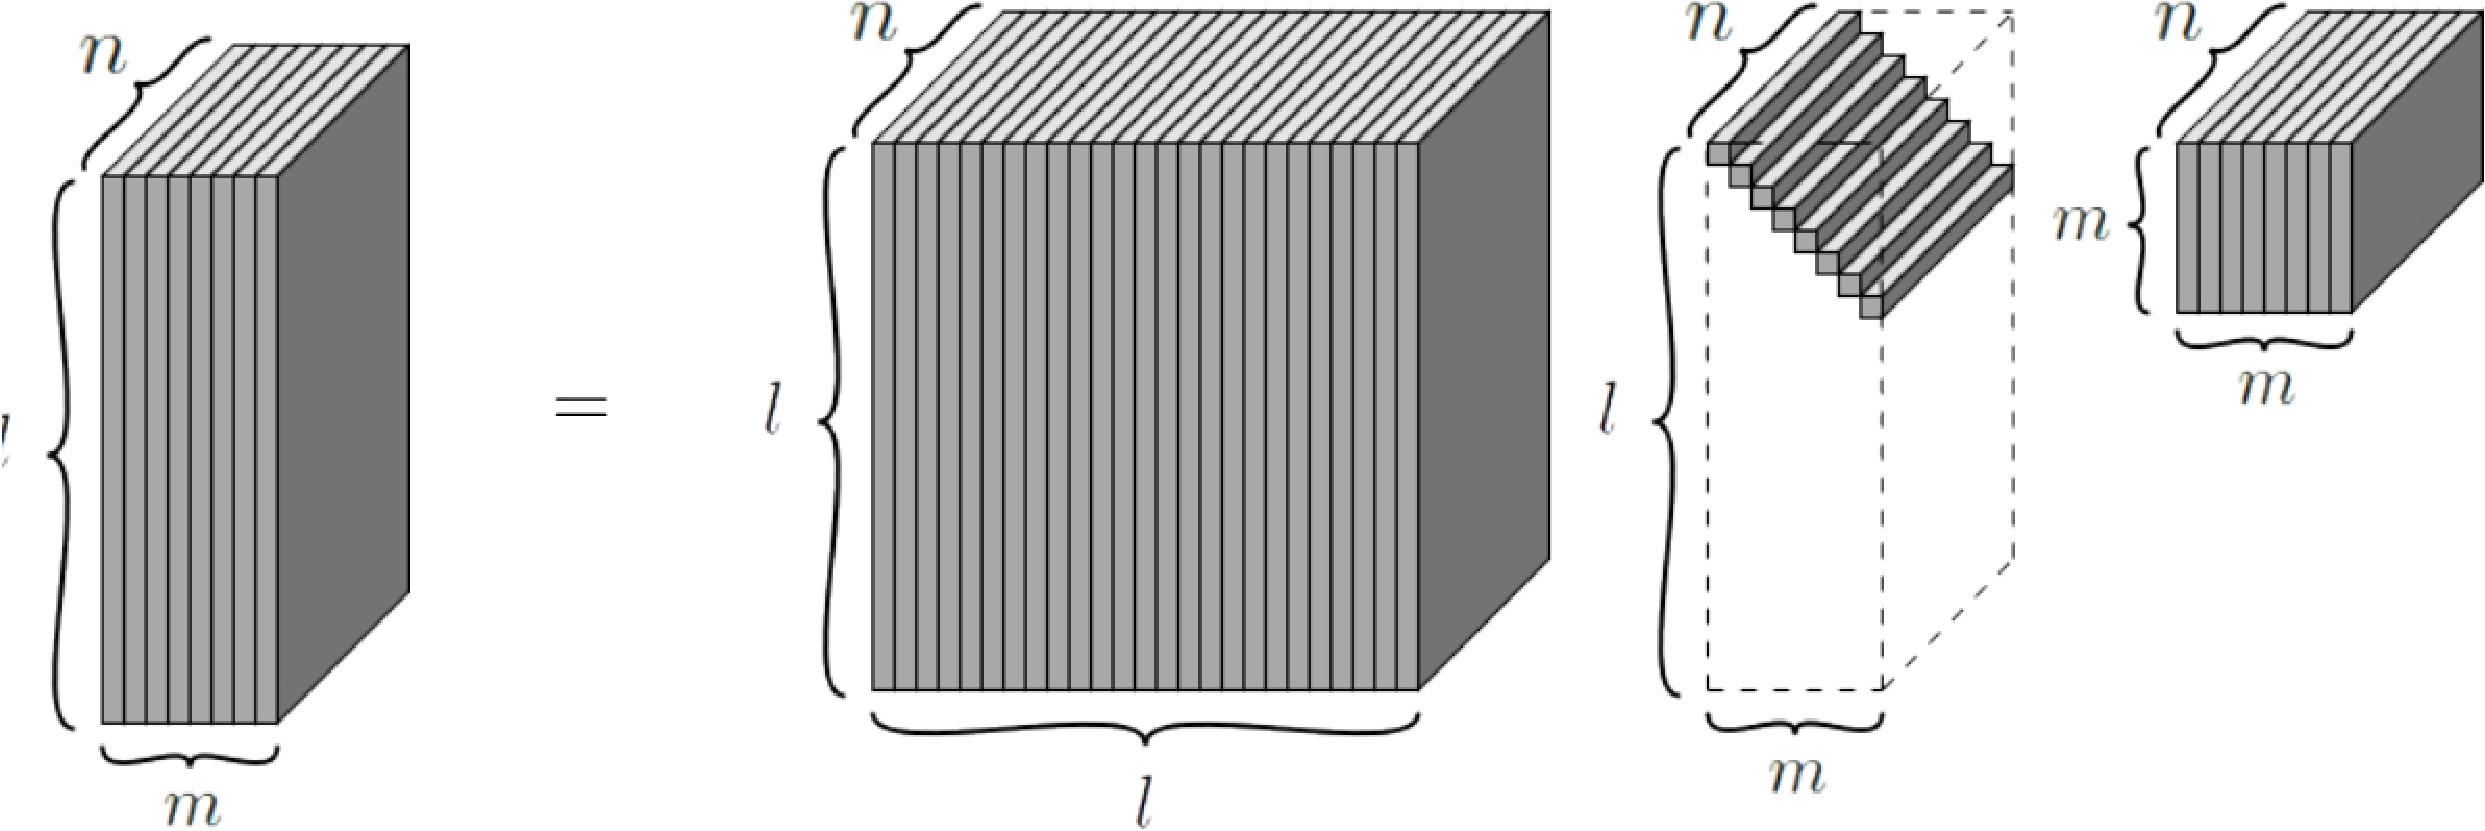
\includegraphics[width=1\textwidth]{img/ok/T-SVD.pdf}
\end{center}
\end{frame}
\begin{frame}
الگوریتم $t-SVD$ برای تانسور سه بعدی به صورت زیر است:
\begin{center}
	
\includegraphics[width=0.8\textwidth]{img/ok/AT-SVD.pdf}
\end{center}
\end{frame}
\begin{frame}

	1 تعریف معین مثبت. 
	\\
	
	\pause
	2 تانسور متعامد\\
	
	\pause
	3 $squeenz$

\pause
\begin{center}
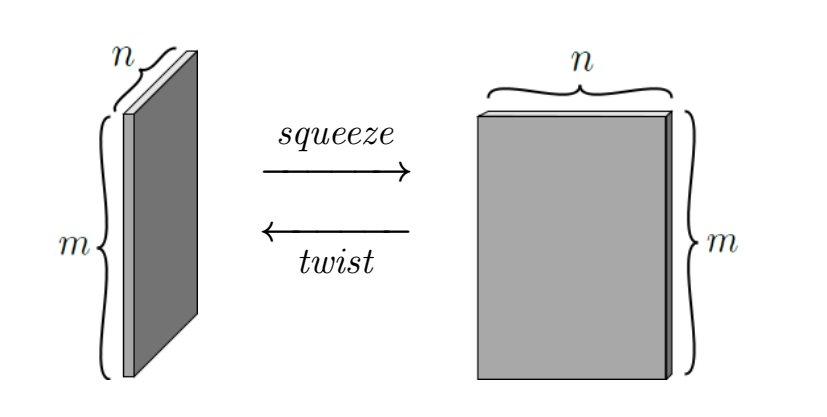
\includegraphics[width=0.8\textwidth]{img/sq.png}
\end{center}
\end{frame}
\begin{frame}{ضرب داخلی}
4 ضرب داخلی برای
$<x,y>:=x^T\star y$

\pause
\begin{center}
	
\includegraphics[width=0.8\textwidth]{img/in.png}
\end{center}
\end{frame}
\begin{frame}{کاربرد $TSVD$}
\begin{center}

\includegraphics[width=0.8\textwidth]{img/tnn.png}
\end{center}
\end{frame}


\section{نتیجه گیری}

\begin{frame}{...}

  \begin{center}\ccbysa\end{center}

\end{frame}

\begin{frame}[standout]
  سوال؟
\end{frame}




\end{document}
